\documentclass[11pt]{article}
\usepackage[a4paper,margin=2.2cm]{geometry}
\usepackage{amsmath,amssymb,booktabs,graphicx,float,xcolor,enumitem,hyperref,tikz}
\usetikzlibrary{arrows.meta,positioning}
\usepackage[T1]{fontenc}
\usepackage{lmodern}
\setlist{itemsep=2pt,topsep=3pt}
\definecolor{boxbg}{RGB}{236,242,250}
\definecolor{warnbg}{RGB}{252,244,228}
\newcommand{\key}[2][boxbg]{\par\medskip\noindent\colorbox{#1}{\parbox{\dimexpr\linewidth-2\fboxsep}{#2}}\par\medskip}
\newcommand{\fig}[3][0.95]{\begin{figure}[H]\centering\includegraphics[width=#1\linewidth]{figures/#2}\caption{#3}\end{figure}}
\newcommand{\x}{\mathbf{x}}

\title{Finding the best voltages with few images:\\ the fleet model, Bayesian optimisation and the validity gate}
\author{ccd\_opt\_ml}
\date{17 November 2026}

\begin{document}
\maketitle

\key{\textbf{In one paragraph.} Each image of a CCD takes about 10 minutes; a trace takes 0.2\,s. To find the voltage
setting that gives the lowest noise and dark charge on a new amplifier, we want as few images as possible. Three tools do
it. (1) A \emph{fleet model} learns, from amplifiers already measured, how noise and dark charge respond to the 18
voltages. (2) \emph{Bayesian optimisation} uses that model to choose the next setting to image, and updates the model after
each image. (3) A \emph{validity classifier} predicts which settings would give an unusable image and forbids them. In a
replay on the v3 data (board 101), these reach a setting within 2\,\% of the best in about 1.3--2.7 images, never imaging a
broken setting; tuning by hand from a random start needs 11--27 images and wastes 3--4.}

\tableofcontents

% =====================================================================================================================
\section{The problem}
A CCD amplifier is operated with 18 voltages (substrate VSUB, output drain VDD, reset drain VR, the reset, summing-well and
output gates, the vertical and horizontal clocks, the transfer gate). Each choice of the 18 values is a \emph{setting}
$\x$. For each setting an image gives three numbers: the read noise $\sigma_e$, the dark charge $\lambda$ and the gain.
Some settings break the readout altogether (the electron peaks merge, most columns turn hot): such an image is
\emph{unusable}.

We want the setting with the lowest noise and/or dark charge. We combine them into one number to minimise,
\begin{equation}
J(\x) = w\,\ln\sigma_e(\x) + (1-w)\,\ln\lambda(\x),
\end{equation}
with $w=1$ for noise only, $w=0$ for dark charge only and $w=0.5$ for both. Logarithms make a 10\,\% change count the same
at any level.

The difficulty: every evaluation of $J$ costs an image (about 10 minutes), the space has 18 dimensions, and about 22\,\% of
the v3 settings were unusable. Trying settings one by one is slow; trying them at random is slower.

\paragraph{What is cheap.} A \emph{trace} (0.2\,s of the raw output at a setting) is cheap enough to take at every
candidate. It measures the amplifier's noise directly and shows a broken readout, but it cannot see charge, so not the
dark charge (amp\_phys reports).

% =====================================================================================================================
\section{Learning a response from data: Gaussian-process regression}
\subsection{The idea}
We do not know the function $J(\x)$. We know it at the settings already imaged. A \emph{Gaussian process} (GP) is a way
to say ``$J$ is some smooth function; here is my best guess of it everywhere, and here is how unsure I am'', and to update
both as measurements arrive.

Before any data, the GP describes a family of smooth random functions (Figure~\ref{fig:basics}, left). Each measurement
pins the function down near that setting: the best guess (the \emph{mean}) passes close to the measured values, and the
uncertainty shrinks there and stays large far from any measurement (middle, right).
\fig{gp_basics.png}{Left: before any measurement, a GP describes smooth functions within a band. Middle and right: after 2
and 5 measurements (orange), the mean (blue) follows the data and the uncertainty band (±2 standard deviations) narrows
near them. The dashed line is the unknown truth.\label{fig:basics}}

\subsection{The formula}
A GP is defined by a \emph{mean} $\mu$ (a constant here: the average $J$) and a \emph{covariance} $k(\x,\x')$: how strongly
the values at two settings move together. We use the Matérn-5/2 covariance
\begin{equation}
k(\x,\x') = s^2\,M(r),\qquad M(r) = \left(1+\sqrt5\,r+\tfrac53 r^2\right)e^{-\sqrt5\,r},\qquad
r = \sqrt{\sum_{i=1}^{18}\left(\frac{x_i-x'_i}{\ell_i}\right)^2}.
\end{equation}
$M=1$ for identical settings and falls towards 0 as they move apart. Its parameters:
\begin{itemize}
\item $\ell_i$, the \textbf{length scale} of voltage $i$: how far that voltage must move before $J$ changes appreciably.
  A short $\ell_i$ means the voltage matters a lot; a long one means it barely matters (Figure~\ref{fig:ls}).
\item $s^2$: how much $J$ varies over the settings.
\item $n^2$: the measurement noise (the repeatability of one image), added on the diagonal.
\end{itemize}
\fig{lengthscale.png}{The same five measurements with three length scales: too short (the guess returns to the mean
between points), about right, too long (too smooth to follow the data). Training picks the length scales that make the
measurements most probable.\label{fig:ls}}

\paragraph{Prediction.} Put the measured values in a vector $\mathbf y$ and their covariances in a matrix $K$
($K_{jk}=k(\x_j,\x_k)$). For a new setting $\x_*$, let $\mathbf k_*$ be its covariance with each measured setting. Then
\begin{align}
m(\x_*) &= \mu + \mathbf k_*^{\!\top}(K+n^2I)^{-1}(\mathbf y-\mu), \label{eq:mean}\\
v(\x_*) &= s^2 - \mathbf k_*^{\!\top}(K+n^2I)^{-1}\mathbf k_*,\qquad \text{uncertainty } s_*=\sqrt{v}. \label{eq:var}
\end{align}
Equation~\eqref{eq:mean} is a \textbf{weighted average of the measured values}: settings similar to $\x_*$ get large
weights. Equation~\eqref{eq:var} says the uncertainty starts at $s^2$ and is reduced by every similar measurement.

\subsection{Training: what is fitted}
There are no weights or layers to train. \textbf{Training means choosing the few numbers $s^2$, $n^2$ and
$\ell_1\dots\ell_{18}$} so that the measured values are as probable as possible under the GP. That probability (the
\emph{marginal likelihood}) is
\begin{equation}
\ln p(\mathbf y) = -\tfrac12(\mathbf y-\mu)^{\!\top}(K+n^2I)^{-1}(\mathbf y-\mu) - \tfrac12\ln\det(K+n^2I) + \text{const}.
\end{equation}
The first term rewards fitting the data; the second penalises a needlessly flexible function. A numerical optimiser finds
the maximum. After that the data themselves, through equations~\eqref{eq:mean}--\eqref{eq:var}, \emph{are} the model.

% =====================================================================================================================
\section{Learning across amplifiers: the fleet model}
\subsection{One model for many amplifiers}
Every amplifier responds to the voltages in a similar way, but each has its own level (one is noisier, one has more dark
charge). The \emph{fleet model} (a multi-task GP) writes, for amplifier $a$,
\begin{equation}
J_a(\x) = \underbrace{f(\x)}_{\text{shared response}} + \underbrace{c_a}_{\text{own level}} + \underbrace{g_a(\x)}_{\text{own deviations}},
\end{equation}
which corresponds to the covariance between an image of amplifier $a$ at $\x$ and one of amplifier $a'$ at $\x'$:
\begin{equation}
K = s^2 M(\x,\x')\left[\rho + (1-\rho)\,\mathbb 1(a=a')\right] + c^2\,\mathbb 1(a=a') + n^2\,\mathbb 1(\text{same image}).
\end{equation}
Two new numbers: $\rho$, \textbf{how alike two amplifiers' shapes are} (1 = identical), and $c^2$, \textbf{how much their
levels differ}. Both are fitted on the fleet with the same likelihood, by comparing the fleet's amplifiers with each other.
The \emph{fleet} is every amplifier already measured; the amplifier being tuned is the \emph{new} one.

\subsection{A real example}
Figure~\ref{fig:train} shows the fleet model with one voltage (VSUB) and one output (dark charge), trained on 200 images of
the two fleet amplifiers 101:0 and 101:1 and used for the hidden amplifier 101:3. The fitted numbers: $s=0.5$ (in
$\ln\lambda$), $\ell_\text{VSUB}=22.6$\,V, $n$ about 31\,\% (large here because the other 17 voltages also moved and this
one-voltage example ignores them), $\rho=0.50$, $c$ about 16\,\%.
\fig{gp_training_example.png}{Fleet model, one voltage. Grey: the fleet's images (training data). Orange: the hidden
amplifier's true values. Left: with no image of it, the prediction (blue) follows the fleet's shape; the level is unknown.
Right: one image of it (star) shifts the whole curve up.\label{fig:train}}

\subsection{Why no image of the new amplifier is needed to choose a setting}
With no image of amplifier $a$, its offset $c_a$ is unknown: the prediction is the shared shape $f(\x)$ with a wider
uncertainty. \textbf{A constant offset does not change which setting is lowest}, so the ranking of settings is already
right if the shapes agree ($\rho$ close to 1). In Figure~\ref{fig:train} (left) the predicted best is the lowest VSUB,
where 101:3 is indeed lowest, while its level is underestimated.

The first image of the new amplifier then fixes its level: all its predictions share the $c^2$ term with that image, so
the whole curve moves (Figure~\ref{fig:train}, right). Later images reveal where its shape departs from the fleet's.
The model trusts one image only as far as $c^2$ allows: if the new amplifier differs from the fleet more than the fleet's
amplifiers differ from each other, it takes a few images to catch up (visible in the figure).

% =====================================================================================================================
\section{Choosing the next image: Bayesian optimisation}
\subsection{The loop}
\begin{enumerate}
\item Predict $m(\x)$ and $s(\x)$ for every candidate setting with the fleet model (fleet images + the new amplifier's
  images so far).
\item Compute the \textbf{expected improvement} of each candidate (below) and image the best one.
\item Add the image to the data and go back to 1. Stop when no candidate is expected to improve on the best image by more
  than the measurement repeatability.
\end{enumerate}

\subsection{Expected improvement}
Let $b$ be the best (lowest) $J$ imaged so far on the new amplifier. Imaging $\x$ improves on it by $\max(0,\,b-J(\x))$.
The model gives $J(\x)\sim\mathcal N(m,s^2)$, so the expected improvement is
\begin{equation}
\mathrm{EI}(\x) = (b-m)\,\Phi(z) + s\,\varphi(z),\qquad z=\frac{b-m}{s},
\end{equation}
with $\Phi$, $\varphi$ the standard normal distribution and density. EI is large where the prediction is good ($m$ well
below $b$: \emph{exploit}) or where the model is unsure ($s$ large: \emph{explore}). Figure~\ref{fig:ei} shows how this
picks a setting next to the best image, on the side where the model is unsure.
\fig[0.75]{expected_improvement.png}{Top: the model after three images. Bottom: the expected improvement; its maximum is
the next image. It sits beside the current best, where the predicted value is low and the uncertainty still
large.\label{fig:ei}}

% =====================================================================================================================
\section{Never imaging a broken setting: the validity classifier}
About 22\,\% of the v3 settings gave unusable images. A \textbf{classifier} learns which: extremely randomised trees (300
decision trees, each splitting the settings at random thresholds), trained on every image's outcome, usable or not.
Its output $P(\text{usable}\mid\x)$ is the fraction of trees voting ``usable''. Inputs: the 18 voltages, and in the trace
variants also the trace features of the candidate.

Two ways to use it:
\begin{itemize}
\item \textbf{Soft}: maximise $\mathrm{EI}(\x)\times P(\text{usable}\mid\x)$. A broken setting can still win if its EI is
  huge, and broken settings often have unusual traces, which the GP sees as uncertain and so promising.
\item \textbf{Hard gate}: never image a candidate with $P<0.5$. Implemented, this removed almost all wasted images
  (Section~\ref{sec:results}).
\end{itemize}
On its own (sealed session H, new amplifier) the classifier ranks usable above unusable almost perfectly (AUC 0.99); at
$P<0.5$ it catches 18 of 20 unusable settings when it sees the traces, about 10 of 20 from the voltages alone, and flags
no usable setting.

% =====================================================================================================================
\section{Using the traces}
\begin{itemize}
\item \textbf{Trace features as model inputs}: the BO model also receives physics features of each candidate's trace
  (white and 1/f noise, predicted 500-skip noise, gain signals). On v3 this did not speed up the search: within one
  amplifier and one night, these features are either mostly repeat noise (white level: 100\,\% repeat noise; 1/f level:
  70\,\%) or precise copies of what the voltages already say (the reset and summing-well signals). They identify the
  \emph{amplifier}, not the better \emph{setting}.
\item \textbf{Trace-driven ranking}: noise predicted from each candidate's own trace (a tree model trained on the fleet,
  as in the noise test that reached 8.6\,\% absolute error on a new amplifier), dark charge from the fleet model, the
  validity gate, and images only to confirm, in that order. No image guides it.
\item \textbf{Hybrid}: the trace-driven top pick is the first image; fleet BO with the gate continues from there.
\end{itemize}

% =====================================================================================================================
\section{How the strategies were tested: replay on v3}
\subsection{The replay}
The v3 data (board 101, amplifiers 0, 1, 3; 381 images over sessions G and H, 82 of them unusable) are replayed as if
tuned live:
\begin{itemize}
\item Each amplifier in turn is the \emph{new} one; the \emph{fleet} is the other two, from a different half of the night
  (time block), so the new amplifier never shares a moment with its training data.
\item The \emph{candidates} are the new amplifier's measured settings in one block (about 50--65). ``Imaging'' a candidate
  reveals its measured $J$ (and whether it was usable).
\item Score: after each image, how far the best usable $J$ found so far is above the best usable $J$ of the pool, in \%.
  ``Images to 2\,\%'' is the first image count where that gap is at or below 2\,\%. Each number is the mean of 6 searches
  (3 amplifiers $\times$ 2 blocks); differences below about one image are not meaningful.
\item Wasted images: unusable images taken before the 2\,\% point.
\end{itemize}

\subsection{The baselines}
\begin{itemize}
\item \textbf{Random order}: the candidates in random order (average of 200 orders).
\item \textbf{A person}: start at nominal (or at a random setting) and \emph{hill-climb}: always image the untested setting
  closest to the best so far (in standardised voltages). The replay can only step between measured settings, which move
  all voltages at once, so this approximates working outward, not one-knob-at-a-time tuning.
\item \textbf{Fleet ranking, no updates}: the candidates in the order the fleet model predicts, no learning.
\item \textbf{BO without the fleet}: the same loop with only the new amplifier's own images.
\end{itemize}

\subsection{Pitfalls found and fixed along the way}
\key[warnbg]{\textbf{Failed fits as ``best settings''.} Three v3 images that passed the image-fit check had
$\lambda\approx0.0007$\,e/pixel (failed dark-charge fits, 400$\times$ below normal). In log units they were the ``best
settings'' of their pools, and early results rewarded strategies that found them. Fit results below 0.005\,e/pixel are now
treated as unusable.\\[3pt]
\textbf{Hidden reference images.} The default labels are corrected for drift during the night using each amplifier's
nominal reference images, including the new amplifier's. Runs without that correction (no reference image of the new
amplifier at all) are reported separately.\\[3pt]
\textbf{Broken settings are candidates.} In reality a setting's usability is unknown until imaged, so unusable settings
stay in the pools and cost an image when chosen.}

% =====================================================================================================================
\section{Results}\label{sec:results}
\begin{table}[H]\centering\small
\caption{Images to reach within 2\,\% of the best usable setting (wasted unusable images in brackets). v3, every setting in
the pools, mean of 6 searches.}
\begin{tabular}{lccc}\toprule
 & noise only & noise + dark charge & dark charge only\\\midrule
\multicolumn{4}{l}{\textit{Nominal setting known (one nominal image to start)}}\\
Person: hill-climb from nominal & \textbf{1.5} (0) & 26.8 (4.3) & 26.0 (4.5)\\
Random order & 5.0 (0.9) & 31.0 (4.7) & 38.0 (5.7)\\
Fleet ranking, no updates & 3.7 (0.2) & 9.2 (1.0) & 9.2 (1.0)\\
Trace-driven & 1.7 (0) & 8.3 (0) & 8.2 (0)\\
Fleet BO + hard gate & 3.7 (0) & \textbf{2.5} (0) & \textbf{2.7} (0)\\
Hybrid & 3.0 (0) & 2.8 (0) & 2.7 (0)\\
BO without the fleet & 5.8 (1.0) & 4.8 (0.7) & 4.8 (0.7)\\\midrule
\multicolumn{4}{l}{\textit{Nothing known (no nominal, no image of the new amplifier)}}\\
Person: hill-climb from a random start & 11.5 (4.4) & 24.0 (3.1) & 26.8 (3.4)\\
Random order & 6.5 (1.5) & 31.0 (4.8) & 38.5 (5.7)\\
Fleet ranking, no updates & 4.3 (0.5) & 8.3 (1.0) & 8.3 (1.0)\\
Trace-driven & \textbf{1.3} (0) & 7.7 (0) & 7.3 (0)\\
Fleet BO + hard gate & 3.5 (0.2) & \textbf{1.7} (0) & \textbf{1.8} (0)\\
Hybrid & 2.8 (0) & 2.2 (0) & \textbf{1.8} (0)\\
BO without the fleet & 8.2 (2.2) & 3.2 (0.3) & 4.0 (0.5)\\\midrule
\multicolumn{4}{l}{\textit{No reference image of the new amplifier at all (no nominal, no drift correction)}}\\
Fleet's predicted best, then hill-climb & \textbf{2.2} (0.3) & 5.3 (0.3) & 14.8 (3.0)\\
Fleet BO + hard gate & 5.3 (0.3) & \textbf{2.2} (0) & \textbf{2.0} (0)\\\bottomrule
\end{tabular}\end{table}

\fig{search_curves.png}{How the best image found so far approaches the best usable setting, nothing known (no nominal
image). The dotted line is the 2\,\% threshold.\label{fig:curves}}

\paragraph{Reading the results.}
\begin{itemize}
\item \textbf{Noise}: if nominal is known, working outward from it by hand is best (1.5 images): on v3 nominal is already in
  the low-noise region. If nothing is known, the trace-driven ranking is best (1.3 images), because each candidate's trace
  measures its noise.
\item \textbf{Dark charge counts}: fleet BO with the hard gate is best (1.7--2.7 images). By hand it takes 24--38 images,
  because the best dark charge (low VSUB) lies far from nominal and stepping there takes long.
\item \textbf{The hybrid} is never worse than 3 images in any case: one procedure for every objective.
\item \textbf{Tighter thresholds}: reaching the measured best itself takes about 2.5--3.5 images for dark-charge objectives
  (fleet BO + gate) and 5 for noise (trace-driven); below about 2\,\% for noise, ``the best'' is partly measurement luck
  (repeatability 1.5--2\,\%).
\item \textbf{Across two nights} (v2 + v3) the picture is less clean: the trace features shift between nights and the
  fleet's prior misled one objective (16--18 images). A per-night setup covariate (a static noise record) is the fix to try.
\end{itemize}

% =====================================================================================================================
\section{The live procedure}
In a live search there is no pool of measured settings; candidates are generated. The script
\texttt{lvl1/propose\_next.py} does one round at a time and writes packet plans that \texttt{run\_plan.sh} (in
\texttt{daq\_scripts/}) runs:
\begin{center}
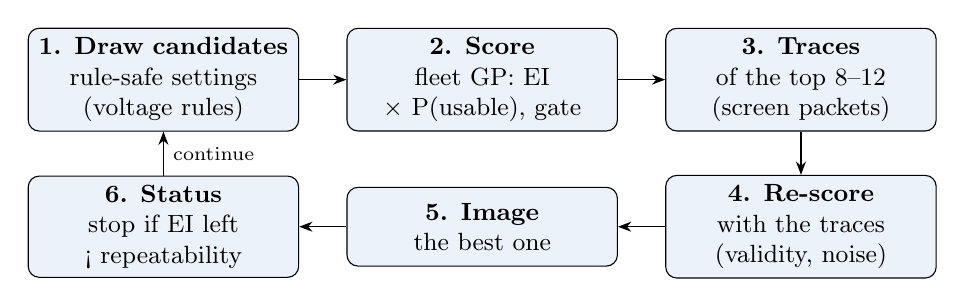
\begin{tikzpicture}[node distance=0.55cm and 0.6cm, box/.style={draw,rounded corners,fill=boxbg,align=center,font=\small,minimum height=1.0cm,text width=3.2cm}, >=Stealth]
\node[box] (a) {\textbf{1. Draw candidates}\\rule-safe settings\\(voltage rules)};
\node[box,right=of a] (b) {\textbf{2. Score}\\fleet GP: EI\\$\times$ P(usable), gate};
\node[box,right=of b] (c) {\textbf{3. Traces}\\of the top 8--12\\(screen packets)};
\node[box,below=of c] (d) {\textbf{4. Re-score}\\with the traces\\(validity, noise)};
\node[box,left=of d] (e) {\textbf{5. Image}\\the best one};
\node[box,left=of e] (f) {\textbf{6. Status}\\stop if EI left\\< repeatability};
\draw[->] (a)--(b); \draw[->] (b)--(c); \draw[->] (c)--(d); \draw[->] (d)--(e); \draw[->] (e)--(f);
\draw[->] (f)--node[right,font=\scriptsize]{continue}(a);
\end{tikzpicture}
\end{center}
\begin{enumerate}
\item \texttt{propose\_next.py screen}: draws hundreds of settings that pass the voltage windows and rules
  (\texttt{docs/voltage\_rules.txt}, \texttt{configs/limits.toml}, with margins, reset-safe and rampable), scores them with
  the fleet model and the classifier, and writes the best as trace-only packets.
\item After the traces: \texttt{amp\_phys/physics\_features.py} and \texttt{gain\_features.py} on them, then
  \texttt{propose\_next.py image}, which re-scores with the trace-informed classifier and writes the image packet.
\item \texttt{propose\_next.py status}: the largest expected improvement left against the repeatability; STOP or CONTINUE.
\end{enumerate}
Tested on v3 (dry run): on the fully explored board 101 it reports STOP (0.25\,\% left); treating amplifier 101:3 as never
seen, it proposes 8 rule-safe screens with $P(\text{usable})$ 0.89--0.97.

% =====================================================================================================================
\section{Limits and next steps}
\begin{itemize}
\item \textbf{The ``new'' amplifier is a sibling}: same board, CCD module and night as the fleet, which share the voltage
  response almost exactly. A different CCD may differ more in shape; then more images are needed early and the traces
  matter more. The decisive test is a live run on a CCD the fleet has not seen.
\item \textbf{Small numbers}: 6 searches per entry; repeated runs or more blocks would tighten the comparisons.
\item \textbf{Replay versus live}: the replay can only pick measured settings; the live loop can propose new ones.
\item \textbf{Improvements to try}: keep the trace-predicted noise in the model at every step of the hybrid; a per-night
  setup covariate; a strip (about a minute) as an intermediate step for dark charge; returning the noise/dark-charge
  trade-off curve instead of one weighting.
\end{itemize}

\appendix
\section{Code and results}
\begin{itemize}
\item \texttt{lvl1/fleet\_tests.py}: the fleet model (\texttt{MultiTaskGP}), the replay (\texttt{bo}), few-shot and
  residual tests. Options used: \texttt{--include-invalid --gate 0.5 --trace-driven --start none|nominal --drift}.
\item \texttt{lvl1/propose\_next.py}: the live procedure.
\item \texttt{amp\_phys/physics\_features.py}, \texttt{gain\_features.py}: the trace features.
\item Result tables: \texttt{amp\_phys/results/fleet\_bo/} (all variants, thresholds 0--5\,\%, wasted images).
\item Figures: \texttt{docs/overleaf\_bo\_fleet\_2026-11-17/make\_figures.py}.
\end{itemize}
\end{document}
